%auto-ignore
%      this ensures the arxiv doesn't try to start TeXing here.
%!TEX root = super_lattice_models_draft.tex
%      prev line helps TeXShop do the right thing




%%%%%%%%%%%%%%%%%%%%%%
\section{Super pivotal categories}  \label{def_sect}
%%%%%%%%%%%%%%%%%%%%%%

In this section we give a more formal (though not completely formal) definition of super pivotal categories.
Since the usual bosonic case is well covered in the literature, we will concentrate on
the differences between the bosonic case and the fermionic/super case.
We will also fix some notation and conventions used elsewhere in the paper.


There are various ways of axiomatizing string nets, including Kuperberg spiders \cite{kup_spider}, 
planar algebras \cite{jones_pa},
disk-like 2-categories \cite{blob_paper}, and pivotal tensor categories \cite{Joyal1991}.
\kwx{Is this the earliest reference?  Maybe Joyal and Street?}
\davex{This one \cite{Joyal1991}? (I haven't read it).}
\kwx{That's probably it; see also the two references at the end of the wikipedia article: https://en.wikipedia.org/wiki/Dual\_object;
if it were up to me, I would not do further citation research and just go with the JS citation you already have.}
%\dave{Should we cite \cite{Barrett1999}?}
\davex{That's fine with me.}

The first three are better suited to our applications, but the last one is likely the most familiar to a majority or our readers,
so we will describe a fermionic/super version of pivotal tensor categories.

So far as we know, the earliest definition of a super pivotal tensor category was given in \cite{blob_paper}.
In the higher category definition given in that paper, one of the parameters was the type of balls used to 
specify morphism spaces.
If we take those balls to be 2-dimensional and equipped with spin structures, then one has a definition of a super pivotal 2-category.
We can then take a super pivotal tensor category to be a super pivotal 2-category with only one 0-morphism.
The more traditional-style definition given below is reverse-engineered to be
equivalent with the definition already contained in \cite{blob_paper}.

\medskip

Recall from 
\cite{Joyal1991}
\kwx{change this ref if we change the earlier one}
that the data of a pivotal category includes:
\begin{itemize}
\item A set of objects $\spc^1$.
\item A set of morphisms $\spc^2$.
\item A binary operation $\otimes$ (horizontal composition) on objects and morphisms.
\item A binary operation $\circ$ on morphisms.
\item A pivotal structure $*$ defined on both objects and morphisms.
\end{itemize}


The definition of a super pivotal category differs from the usual bosonic case in the following ways:

\begin{enumerate}
	\item The space of morphisms between two objects has the structure of 
	a super vector space.
	Morphisms also satisfy the {\em super interchange law} \cite{brundan2016}:
	\begin{align}
	(f_1\tp f_2) \circ (g_1\tp g_2) = (-1)^{|f_2| |g_1|} (f_1\circ g_1)\tp (f_2\circ g_2)
	\end{align}
	where $|f|$ is the parity of the morphism $f$. 
	\item There are two distinct types of simple object, ``m-type" and ``q-type".
	m-type simple objects have trivial endomorphism algebras $\cc$, as is the case in bosonic theories.  
	%m-type simple objects have the same properties as objects in conventional (bosonic) fusion categories, and have trivial endomorphism algebras $\cc$.  
	q-type simple objects have endomorphism algebras isomorphic to $\cliff_1$, 
	and so their endomorphism algebras contain odd elements in addition to scalars. (See Section \ref{def_sob_ss}.)
	\item In order to keep track of Koszul signs arising from exchanging fermions, 
	we must keep track of a sign-ordering of individual fusion spaces (See \ref{koszul_signs}).
	\item Fusion spaces $V^{abc}$, $V^{ab}_c$, $V_{abcd}$, etc.\ are not merely supervector spaces; they come equipped with an action of the
	endomorphism algebras of the objects being fused. 
	For example, $V^{abc}$ possess an action of $\End(a)\tp \End(b)\tp \End(c)$.
	(See \ref{fusion_spaces}.)
	\item When combining basic 3-valent fusion spaces $V^{ab}_c$ to form fusion spaces of higher valence, we must take
	tensor products over the endomorphism algebras of the simple objects which connect two fusion spaces. 
	For example, we form the fusion space $V^{ab}_{cd}$ as $V^{ab}_{cd} \cong \bigoplus_e V^{ab}_e \tp_{\End(e)} V^e_{cd}$.
	If $e$ is m-type, this is just the usual tensor product over $\cc$, as in the bosonic case.
	But if $e$ is q-type, then we must take a non-trivial tensor product over $\cliff_1$.
	(See \ref{modified_tensor_product}.)
	\item The square of the pivotal anti-automorphism is 
	the fermion parity functor $(-1)^F$, rather than the identity functor (see \ref{pivotal_structure}). 
	If $*$ is the pivotal anti-automorphism, then 
	\be f^{**} = (-1)^{|f|}f.\ee
	In order to keep track of minus signs that result from rotating fermions by $2\pi$, we must keep track of a spin-framing at each fusion space. 
	\item The coherence equations for the basic data of the theory (e.g.\ the pentagon relations) are modified to incorporate  
	 Koszul signs resulting from reordering various fusion spaces. 
	 They are also modified to incorporate the tensor products over endomorphism algebras mentioned above. (see \ref{Fsymbols})
	\item In order to define an inner product, we need to equip the manifold on which our string-nets are 
	defined with a $pin_\pm$ structure, which is discussed in Appendix \ref{fermion_line_bundle}.
\end{enumerate}

%\kw{We should include some figs, either here or later in this section when we go into more detail.}
%\dave{Agreed. Lets do it later in the section as we go over each point.}




%%%%%%%%%%%%%%%
\subsection{Simple objects}  \label{def_sob_ss}
%%%%%%%%%%%%%%%

We will assume that our category $\spc$ is {\it idempotent complete} -- 
every idempotent is the identity morphism of an associated object.
We also assume that $\spc$ is {\it additive} -- we can take direct sums of objects.

An object $a$ of $\spc$ is called {\it simple} if any homogeneous non-zero endomorphism of $a$ is an isomorphism.
Equivalently, $a$ is simple if it has no quotient objects.
(We also stipulate that the zero object is not a simple object.)

In the usual bosonic, non-super case, the only possible endomorphism algebra for a simple object
is the trivial algebra $\cc$ (scalars).
In the fermionic/super case, there is a second possibility: the complex Clifford algebra $\cliff_1$, 
which is the only nontrivial $\zt$-graded division algebra other than $\cc$.
$\cliff_1$ is generated over $\cc$ by the identity (which is even) and an odd element $f$ such that $f^2 = \lambda \cdot \id$
(or $f^2 = \lambda$ for short) for some non-zero complex number $\lambda$. 
Note that by rescaling the odd generator $f$ we can make $\lambda$ in the definition of $\cliff_1$ any nonzero complex number. 

It follows that simple objects in a super pivotal category fall into two classes, according to whether their endomorphism algebras are $\cc$ or $\cliff_1$. 
These are the m-type and q-type objects discussed earlier. 
A simple object is {m-type} if its endomorphism algebra
is $\cc$, and {q-type} if its endomorphism algebra is $\cliff_1$:
\begin{align}
\vcenter{\xymatrix @!0 @M=1mm @C=25mm{
& \text{End}(x) = \mathbb{C} \ar@{<->}[rr] &   &\text{$x$ is a simple m-type object}&  \\
&\text{End}(x) = \mathbb{C} \ell_1 \ar@{<->}[rr]  &  &\text{$x$ is a simple q-type object}&
	}}
\end{align}
This terminology comes from the notation of \cite{jozefiak1988}, which classifies simple super algebras over $\cc$ as either
$M(p|q) = \End(\cc^{p|q})$ or $Q(n)$ (see appendix \ref{superstuff}).
Note that we are using ``simple" here in two different (and well-established) senses: 
any $M(p|q)$ or $Q(n)$ is a simple super algebra
(because it has no non-trivial ideals), but the endomorphism algebra of a simple object must be either
$M(1|0) \cong M(0|1) \cong \cc$ or $Q(1) \cong \cliff_1$,
because all of the larger $M(p|q)$ or $Q(n)$ contain non-invertible elements.

The existence of q-type particles is responsible for much of the novel physics present after performing fermion condensation. 
q-type objects were also discussed in \cite{usher2016,gaiotto2016}, where they were referred to as ``Majorana objects''. 
%\kw{proposed addition:}
(We prefer the m-type/q-type terminology, since it makes clearer the relationship to the Morita classification of 
simple super algebras.)
%\davex{I like it. Although I really do enjoy saying `semi-simple super algebras' whenever possible.}



%%%%%%%%%%%%%%%%%%%%%%%%%%%
\subsection{Fusion spaces} \label{fusion_spaces}
%%%%%%%%%%%%%%%%%%%%%%%%%%%

Arbitrary morphism spaces in a super pivotal category can be built out of basic fusion spaces
$V^{ab}_c = \mor(c\to a\tp b)$,
where $a$, $b$ and $c$ are simple objects (equivalently, minimal idempotents).
This is a super vector space of dimension
$N^{ab}_c = \dim V^{ab}_c = p|q$, where $p$ is the dimension of the even part
of $V^{ab}_c$ and $q$ is the dimension of the odd part of $V^{ab}_c$.

Alternatively, we can treat $a$, $b$ and $c$ more symmetrically and define
$V^{abc} = \mor(\unit\to a\tp b\tp c)$, a super vector space of dimension $N^{abc}$.
In most of this paper we use $V^{ab}_c$, but in Sections \ref{Super_pivotal_Hamiltonian} and \ref{state_sums} we find it more convenient
to use $V^{abc}$.
Elements of the morphism spaces $V^{abc}$ and $V^{ab}_c$ are depicted by
\begin{align}
\PitchFork{a}{b}{c}{\mu} \quad \quad \quad \text{and} \quad \quad \quad \Nonpitchfork{a}{b}{c}{\mu}.
\end{align}
We call the fusion spaces $V^{abc}$ ``pitchforks" because of their graphical depiction.
Of course we have $V^{ab}_c \cong V^{abc^*}$ (see \ref{pivotal_ss} below).
%\kw{probably should add figs for $V^{ab}_c$ and $V^{abc}$}
%\dave{Done.}

More generally, we define $V^{ab}_{cd} = \mor(c\tp d\to a\tp b)$, $V^{ab}_{cde} = \mor(c\tp d\tp e\to a\tp b)$,
$V_{abcd} = \mor(a\tp b\tp c\tp d\to \unit)$, and so on.
In general, we do not require that the objects $a$, $b$ etc. be simple.

\medskip

It is very important to note that $V^{ab}_c$ is not merely a super vector space -- it also comes equipped with an action
of (i.e.\ module structure for) the endomorphism algebras of $a$, $b$ and $c$, and hence admits an action of $\End(a)\tp \End(b)\tp \End(c)$. 
It is impossible to construct the full super pivotal category without knowing this module structure (see \ref{modified_tensor_product} below), 
so the module
structure is part of the input data.
Note that the module structure implies that $N^{ab}_c = n|n$ if any of $a$, $b$ or $c$ is q-type.
This is because any representation of $\cliff_1$ has equal even and odd dimensions.
Acting with the odd (and invertible) element of $\cliff_1$ gives an isomorphism between the even and odd parts of $V^{ab}_c$, 
and hence they must have the same dimension.

%\kw{This would be a good place to insert a def of $\Gamma$ matrices}
%\dave{OK. We had the following diagrams already made, so I'll use them.
%If we would rather use pitchforks, that's also fine.}
The explicit matrix elements of these isomorphisms can be defined in the following way. 
Let $\psi \in V^{ab}_c$ and suppose that $b$ is a q-type simple object, and let $\Gamma_b \in \End(b)$ be an odd endomorphism.
Then 
\begin{align}
\Gamma_b \left( \Vertexa \right) = \sum_{\eta \in V^{ab}_c} \left[ \Gamma_b \right]_{\psi \eta }\Vertexe, 
\end{align}
where the matrix elements are obtained from 
\begin{align}
\label{Gamma_y_def}
\Gamma_b \left( \Vertexa \right) \; = \; \Vertexb \; =\; \sum_{\eta \in V^{ab}_c} \; \Vertexe \; \left( 
{\Vertexc}\middle/ {\Vertexd} \right), 
\end{align}
where the $\eta^*$ provide a complete orthogonal basis (with respect to the pairing \eqref{reflection_pairing_defn}) for $V^{b^*a^*}_{c^*}$.
%\kw{Don't we need to say that the $\eta^*$ basis is dual/orthogonal to the $\eta$ basis?}
%\dave{Will fix: ``dual with respect to this pairing..."}
If either $a$ or $c$ are q-type, then $\Gamma_a$ and $\Gamma_c$ matrices can be defined in a similar way. 

%%KW this same argument has already been made in a footnote near the beginning of the E6/2 section, so I'm removing it here
\begin{comment} %%%%%%%%%
Requiring that the Hilbert space at a given vertex admit a 
representation of $\End(a)\tp \End(b)\tp \End(c)$ places constraints on the types 
of fermionic theories one can write down. 
For example, we can use this to show that a ``q-type Fibonacci'' theory 
which contains a single q-type particle $\tau$ with the fusion space $V^{\tau\tau}_{\tau}\cong \cc^{1|1}$, cannot exist. 
Indeed, if $V^{\tau\tau}_{\tau}$ is nontrivial and $\tau$ is q-type, 
then we must be able to find a representation of $\End(\tau)^{\tp 3} = \cliff_1^{\tp 3} \cong \cliff_3$ on $V^{\tau\tau}_{\tau}$.
This is impossible if $V^{\tau\tau}_{\tau}\cong \cc^{1|1}$, since $\cc^{1|1}$ is not large enough to represent $\cliff_3$. 
This means that theories which contain a q-type particle $\tau$ with $V^{\tau\tau}_{\tau}\neq0$ must contain nontrivial 
fusion multiplicities, which provide us with fusion spaces that are large enough to admit a representation of $\cliff_3$.
Indeed such a q-type particle exists in the $\halfesix$ theory considered earlier (see Section \ref{halfesix}), 
which possesses nontrivial fusion multiplicities that allow the relevant fusion spaces in the theory to be large enough to represent $\cliff_3$. 
\end{comment} %%%%%%%%%


\medskip

If at least one of $a,b,c$ is q-type, we can simplify the description of $V^{ab}_c$ slightly, 
which we have done when working out the examples considered earlier.
Suppose $c$ is q-type, and that $\{|\psi_i\rangle\} \in [V^{ab}_c]^0, i =1,\dots, r$ are the even basis vectors in $V^{ab}_c$. 
Then we can define a complete set of odd basis vectors $\{ |\eta_i\rangle \}$ for $[V^{ab}_c]^1$ by $|\eta_i\rangle = f|\psi_i\rangle$, where $f$ is the odd element of $\End(c) \cong \cc^{1|1}$.
%%KW: I don't think this is true for non-simple c      (or any odd element in $\End(c)$ if $c$ is not simple).
When we write $|\eta_i\rangle$ graphically, we will write it as $f |\psi \rangle$, which allows us to  ``shift the oddness out of the vertex onto the edge'' by transferring the fermion residing on the fusion space to the q-type particle $c$. 
Graphically, this means that we are allowed to ``displace'' dots from trivalent vertices onto q-type worldlines:
%\be \mathord{\vcenter{\hbox{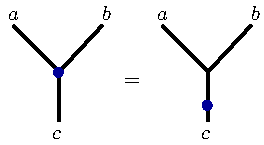
\includegraphics[scale=1]{dot_displacement.pdf}}}}, \ee
\begin{align} \label{dot_displacement} 
\NonPitchforkDot{a}{b}{c}{\eta_i} \;\; = \;\; \NonPitchforkDotDisplaced{a}{b}{c}{\psi_i}
\end{align}
%\kw{should add arrows (edge orientations) to this and similar figs}
%\dave{I'll add arrows to figs as I go through.}
where the picture on the left is $|\eta_i\rangle$ and the one on the right is $f|\psi_i\rangle$, and $c$ is assumed to be q-type. 
Although this is not a deep fact, it proves to be helpful when doing graphical manipulations, 
and operators implementing transformations like \eqref{dot_displacement} will be crucial for writing down the lattice 
Hamiltonian which realizes the
super pivotal version % fermionic generalization 
of the Levin-Wen Hamiltonian. 

\medskip

\dave{Modified this to amend comments as per discussion. 
EL and KW may want to look at it.}
\ethan{made some tiny changes; looks good to me}
Lastly, we will define a non-degenerate bilinear pairing between vectors in the vector space assigned to a disk with $n$ marked points. 
We will focus on fusion spaces of the form $V^{x_1\dots x_n}$, but the construction
for different types of fusion spaces is analogous. 
The pairing is defined by 
\begin{align} \label{reflection_pairing_defn}	% note that there are no reflections involved in defining this pairing, tex label notwithstanding
\mcb:\;  &V^{x_n^* \cdots x_2^* x_1^*} \tp V^{x_1 x_2 \cdots x_n}  \ra \cc \\
\nonumber &\Bilineara \tp \Bilinearb \mapsto \Bilinearc
\end{align} 
%\dave{Koszul signs outside of box, remove subscript $i$ and $j$. (but leave them below).}
%\dave{Maybe more natural to have $\mcb:\; V^* \tp V \ra \cc$ like in quantum mechanics $\bra{x} \tp \ket{y} \mapsto <x,y>$}
%\ethan{I agree, especially since we've done $\chi$ that way}
where $\mu\in V^{x_n^* \cdots x_2^* x_1^*}$ and $\nu  \in V^{x_1 x_2 \cdots x_n}$. 
We are working with the convention that the Koszul ordering of the tensor product increases 
in a left-to-right fashion (indicated by the numbers $1,2$ in the bottom right of \eqref{reflection_pairing_defn}); we will elaborate on this convention in Sec \ref{koszul_signs}. 
This bilinear pairing is just the evaluation map, and is $\cc$-linear in both its arguments. 
It is non-degenerate, meaning that if $\nu_j$ is a complete basis for the fusion space $V^{x_1 x_2 \cdots x_n}$ and $\mu_i$ is a complete basis for the dual fusion space $V^{x_n^* \cdots x_2^* x_1^*} $, then the matrix $\mcb_{ij} = \mcb(\mu_i \tp \nu_j)$ is invertible. 
Hence we can define a set of vectors $\mu_j^* = \sum_i  (\mcb^{-1} )_{ji}\nu_i $ so that
$\mcb( \mu_j^* \tp \mu_i)\propto\delta_{ij}$.
\kw{did you want proportional to $\delta_{ij}$ here?}
\ethan{presumably; I made the change}
\dave{Actually it was intentional due to the previous line. 
We could write  ``...define a set of vectors $\mu_j^* = \Theta(\mu_j^*) \sum_i  (\mcb^{-1} )_{ji}\nu_i $ so that
$\mcb( \mu_j^* \tp \mu_i)= \Theta(\mu_j^*) \delta_{ij}$."
And change below to ``For most of the paper, we will adopt the normalization convention $\Theta(\mu_i) = \sqrt{d_a d_b d_c} $ for $\mu_i \in V^{ab}_c$."}
%In particular, we will make use of the case where for $\mu_i \in V^{c^*b^*a*}$ and $\nu_j^* \in V^{abc}$. 
For most of the paper, we will choose the normalization convention
\begin{align}  \label{b_pairing_defn}
\mcb( \mu_j^* \tp \mu_i )  = \sqrt{d_a d_b d_c} \, \delta_{ij}
\end{align} 
with $\mu_i \in V^{abc}$ and $\mu_j^* \in V^{c^* b^* a^*}$.
\dave{Could replace RHS with $\Theta(\mu_i)$, depending what we write in state sum section.}
\ethan{I think the explicit form is probably better for our purposes here}
\dave{I kind of like the above idea. Remove the propto and put in an explicit normalization, 
then say something like ``For most of the paper we let $\Theta(\mu_i) = \cdots$ so that \eqref{b_pairing_defn}." }
%The pairing satisfies $\mcb(\mu_{i,1} \tp \nu_{j,2}) =  (-1)^{|\mu_i| |\nu_j|} \mcb(\nu_{j,1} \tp \mu_{i,2})$. 
%\ethan{are we sure? I thought we agreed on the symmetry of $\chi$, which 
%is just $\mcb$ with different normalization. e.g. $\mcb(a_1\tp b_2) = (-1)^{|a|}\mcb(b_2\tp a_1) = \mcb(b_1\tp a_2)$?}
%\dave{This caused me endless confusion,
%so no I'm not sure.
%Something is inconsistent: 
%e.g., I thought we agreed that $a_1\tp b_2 = (-1)^{|a| |b|} a_2 \tp b_1 = (-1)^{|a| |b|}  b_1 \tp a_2$ and that $\mcb$ is linear in both $a$ and $b$.
%But then we also agreed that the evaluation of the diagram is symmetric in both $a$ and $b$ (in the way that you said). 
%Which means LHS of the \eqref{reflection_pairing_defn} and the RHS of \eqref{reflection_pairing_defn} transform differently under interchanging $a$ and $b$.
%}
%\kw{We can isotope one diagram into the other by (say) keeping $\nu$ fixed and rotating $\mu$ to the other side.
%Thus we get a Koszul sign and also a rotation sign $(-1)^{|\mu|}$.
%These two signs cancel.
%Let's discuss on skype to be absolutely sure we are correct.}
%\ethan{I totally agree with Kevin. We already came to this conclusion earlier in the former tensor network 
%section. }
%>>>>>>> 2ca819f56d443747cfb8d550e9bdfc5684778be7

%%%%%%%%%%%%%%%%%%%%%%%%%%
\subsection{Pivotal structure}  \label{pivotal_ss}   \label{pivotal_structure} 
%%%%%%%%%%%%%%%%%%%%%%%%%%

The pivotal structure assigns to each object $a$ a dual object $a^*$.
It also provides linear isomorphisms
\be
	P_L : \mor(a \to b\tp c) \to \mor(b^*\tp a \to c)
\ee
and
\be
	P_R : \mor(a\tp b \to c) \to \mor(a \to c\tp b^*)
\ee
for any objects $a$, $b$ and $c$.
These isomorphisms are required to be functorial with respect to $a$ and $c$.
In addition, they are required to be twisted-functorial with respect to $b/b^*$, where we use the 
$*$ functor (defined below) to relate morphisms with domain $b$ to morphisms with range $b^*$.

For objects $a$, we require that $a^{**} = a$ on the nose (strict pivotal).
For morphisms $f : a\to b$, we define $f^* : b^* \to a^*$ by $f^* = P_L(P_R(f))$, diagrammatically by,
\begin{align}
\fstar \; = \; \fPLPR
\end{align}
%\kw{should add fig for this}
%\dave{done.}
(We have implicitly added and then removed some tensor units (trivial objects) here appearing 
in fusion spaces like $V^{aa^*}_\unit$.)
%\dave{Why have we removed tensor units? 
%I thought $V^{b^*b}$ and $V{aa^*}$ were defined without units.}
%\kw{The pivots are defined on $V^{ab}_c$, not $V^a_a$.}
We think of $f^*$ as a $+\pi$ rotation of the morphism $f$.
We have
\be
	(f\cdot g)^* = (-1)^{|f||g|} g^* \cdot f^* .
\ee
In other words, $*$ is a contravariant functor if one takes Koszul signs into account.

For (strict) pivotal bosonic categories, one requires that $**$ is the identity functor, but
in the fermionic case one requires that $**$ is the spin-flip functor $(-1)^F$.
More specifically, we require
\be
\label{spin_flip_functor}
	f^{**} = (-1)^{|f|} f ,
\ee
since $f^{**}$ is a $2\pi$ rotation of $f$.

The part of the pivotal structure most used in calculations is the $+2\pi/3$ rotation on the 
basic trivalent fusion spaces.
We define the ``pivot" $P^{ab}_c : V^{ab}_c \to V^{bc^*}_{a^*}$
as $P_R\circ P_L$.
In terms of diagrams and matrices, this looks like
\begin{align}
P^{ab}_c \left( \;  \PivotYa \; \right) = \PivotYb
\end{align} 
%\dave{Should we use $P(...)$ or $P\circ ....$?}
%\ethan{I think the former}
The Frobenius-Schur indicator $\kappa_a$ is a special case of the pivot and 
defined by $\kappa_a = P^{\unit a}_{a^*}$, which is non-zero if $a\cong a^*$. 
\davex{If the following is correct, I may prefer to write it that way: either $\kappa_a = \tr P^{\unit a}_{a^*}$
or more explicitly as $\kappa_a = \tr \{ P^{\unit a}_{a^*}: V^{\unit a}_{a^*} \to V^{\unit a}_{a^*} \} $ (it's also more clearly `gauge invariant' when written as a trace).
}
\davex{Actually, maybe $\kappa_a = \tr \{ ... \}$ and $\tilde{\kappa}_a = \str \{... \}$.}
%\dave{Will add comment about S-matrix giving Frob-Schur indicator}
%\ethan{I approve of the following proposed addition}
We also note that the modular $S$ matrix gives the square of the Frobenius-Schur indicator.
If $a \cong a^*$ we have $\kappa_a^2 = (S^2)_{aa}$.
For a bosonic theory the Frobenius-Schur indicators are $\pm1$, and this provides no new information. 
But in fermionic theories the oddly self-dual simple objects have Frobenius-Schur indicators of $\pm i$,
and this is detected by the diagonal entries of $S^2$.
The $m_4$ particle in the $\halfesix/y$ theory is an example of this; see \eqref{hE6_S_NN}.
%%KW I don't agree that there are 8 possible FS indicators
%However, for a fermionic theory $S^4 = (-1)^F$, allowing for eight possible Frobenius-Schur indicators.
%\dave{If we're being careful, 
%doesn't that expression depend on vertex normalization $V^{\unit a^*}_{a^*}$?
%Maybe it should be the inner product $\langle \text{id}_a, \text{id}_{a^*} \rangle$ or $\mcb(v_a\tp v_{a^*}) = \kappa_a d_a$ or just define it through $F$-move (which is essentially what the above does).}

%\kw{insert eqn similar to existing one in older pivotal subsection}.
%\dave{done.}
We can similarly define $P^{abc} : V^{abc}\to V^{bca}$. 
In terms of diagrams, 
\begin{align}
\label{Pitchfork_pivot}
P^{abc} \left(  \Pitchforkabc \right ) \;=\;  \Pitchforkabcrot.
\end{align}
%\dave{Changed form  $P^{abc} : V^{abc}\to V^{bca^*}$ to above.}
%\kw{insert similar eqn/fig; this is the pivot we will use for hamiltonian and tensor network}
%\dave{done}
We will usually write simply $P$, since the $a$, $b$ and $c$ are typically clear from context.

Since $P^3$ acts as a $2\pi$ rotation, we have $P^3 = (-1)^F$. Diagrammatically, when acting on $V^{abc}$ this is written 
\begin{align}
P^3 \left(  \Pitchforkabc \right )\; = \; \PivotThreeTimes \; = \;(-1)^F \Pitchforkabc.
\end{align}
%\be\mathord{\vcenter{\hbox{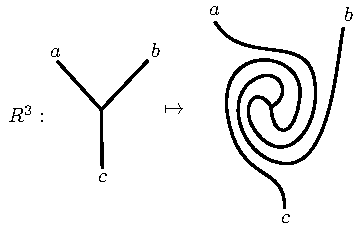
\includegraphics[scale=1]{pivot_cubed.pdf}}}}\ee
%where $\mu \in V^{ab}_c$. 

%\medskip
%\kw{do we need anything else here?}



%%%%%%%%%%%%%%%%%%%%%%%%%%
\subsection{Fusion rules and fusion spaces} \label{fusion_rules_and_fusion_spaces}
%%%%%%%%%%%%%%%%%%%%%%%%%%

%\dave{Minor notational thing: we used $\cdot$ earlier for function composition and for multiplication here. 
%I think it's clear from context what we mean, 
%but am wondering if we should make a note of it.
%}

In this section we elaborate on the differences arising in fermionic theories between fusion spaces and the super vector spaces appearing in the fusion rules. 

We assume that our categories are additively complete, which means that it makes sense to
multiply objects by super vector spaces. 
(This is a categorified version of multiplying vectors by scalars.
Vectors are promoted to objects and scalars are promoted to vector spaces.)
For any collection of super vector spaces $\{W_a\}$ indexed by 
a finite set of objects $\{a\}$ in our category, 
we therefore have an object of the form
\be 
	\bigoplus_a W_a \cdot a .
\ee
%\ethan{moved a sentence to try to provide an explanation of $\cdot$ at Dave's suggestion} where $\cdot$ is the categorified version of multiplying vectors by scalars.

Morphisms between these more general objects are calculated as  
\be  \label{amordef}
	\mor(\bigoplus_a W_a\cdot a \to \bigoplus_b W'_b\cdot b) = \bigoplus_{a,b} \Hom(W_a \to W'_b)\otimes_\cc \mor(a\to b) .
\ee

Because our category is semisimple, there exists a finite collection $\sob(\spc)$ of mutually non-isomorphic simple objects $x$ such
that any object $a$ is isomorphic to one of the form
\be \label{asumx}
	a \cong \bigoplus_{x\in \sob(\spc)} W_x\cdot x .
\ee
If we want the isomorphism to be canonical, we can take $W_x = \mor(x\to a)$ if $x$ is m-type, or $W_x$ to be the even morphisms in $\mor(x\to a)$
if $x$ is q-type.

Combining \eqref{asumx} and \eqref{amordef}, we can compute endomorphisms of objects by
\be
	\End(a) \cong \bigoplus_{x\in \sob(\spc)} \End(W_x) \otimes_\cc \End(x).
\ee

We are now ready to discuss fusion rules. 
For any $a$ and $b$, define the vector spaces $\Delta^{ab}_c$ by
\be
	a \otimes b \cong \bigoplus_{c\in \sob(\spc)} \Delta^{ab}_c \cdot c .
\ee
The $\Delta^{ab}_c$ are the fusion rule coefficients. 

The fusion spaces $V^{ab}_c$ are defined as the vector space of morphisms from $c$ to $a\tp b$:
\be \label{defn_of_V_by_Delta}
	V^{ab}_c = \mor(c \to a\tp b),
\ee
%%KW I don't think we use \equiv elsewhere in the paper
where $a,b,c$ are simple objects. 
Decomposing the tensor product and using the simplicity of $c$, we see that 
\be V^{ab}_c \cong \Delta^{ab}_c \tp \rm{mor}(c \ra c) \cong \Delta^{ab}_c \otimes \End(c).\ee
Thus, the fusion spaces can be larger than the vector spaces appearing in the fusion rules 
(in contrast to bosonic theories, where the fusion spaces and fusion rule coefficients are always equal).
As examples, in the $C_2$ theory studied earlier, we have 
\be \Delta^{q_\sigma q_\sigma}_{m_\psi} \cong \cc^{1|1},\quad\Delta^{q_\sigma m_\unit}_{q_\sigma} \cong \cc,\ee
while 
\be V^{q_\sigma q_\sigma}_{m_\psi} \cong V^{q_\sigma m_\unit}_{q_\sigma} \cong \cc^{1|1}.\ee

$V^{ab}_x$ is cyclically symmetric (up to isomorphism) in $a,b,x$ (if $a$ and $b$ are simple).
Explicitly, this is because 
\be \mor(c \ra a\tp b) \cong \mor(\unit \ra a\tp b \tp c^*) \cong \mor(a^* \ra b\tp c^*),\ee 
which allows us to cyclicly permute the indices of $V$, so long as we take the duals of any objects that move from subscripts to superscripts, and vice versa. 
For example, we have $V^{ab}_c \cong V^{bc^*}_{a^*} \cong V^{c^*a}_{b^*}$. 

On the other hand, $\Delta^{ab}_c$ is {\it not} cyclically symmetric in $a,b,c$, as the $C_2$ theory example shows. 
Additionally, while $V^{ab}_c$ has an action of $\End(a)\otimes\End(b)\otimes\End(c)$ (as mentioned earlier), $\Delta^{ab}_c$
only has an action of $\End(a)\otimes\End(b)$.

%\kw{Maybe this paragraph can be dropped?  We already have a a simpler proof of this fact above.}
%\dave{That's fine with me.
%Ethan, if that's fine with you go ahead and comment it out. 
%An alternative is to put it as a footnote.}
%\ethan{deal}
%This definition of $V^{ab}_c$ gives us another way to show that $V^{ab}_c$ will always be a supervector space of the form $\cc^{n|n}$ for some integer $n$ if any of $a,b,c$ is q-type. 
%Indeed, suppose $c$ were q-type, and $\Delta^{ab}_c \cong \cc^{r|s}$. 
%Then $V^{ab}_c \cong \cc^{r|s} \tp \cc^{1|1} \cong \cc^{r+s|r+s}$. 
%The result then follows by the symmetry of $V^{ab}_c$. 




%%%%%%%%%%%%%%%%%%%%%%%%%%%%%%%%%%
\subsection{Koszul sign rule and unordered tensor products} \label{koszul_signs}
%%%%%%%%%%%%%%%%%%%%%%%%%%%%%%%%%%

We will treat Koszul signs as in \cite[Section 1.2]{deligne1999}.
%\kw{Section 1.2 of Chapter 1 of Volume 1 of the IAS "Quantum Fields and Strings" books.}
This approach doesn't really do away with Koszul signs.
Rather, it pushes them to the background, where they don't need to be mentioned as frequently.
For explicit calculations, they must again be brought to the foreground.

Let $I$ be a finite (and unordered) index set.
For each $i\in I$, let $W_i$ be a super vector space.
We define the unordered tensor product,
\be
	\bigotimes_{i\in I} W_i ,
\ee
as follows.
For each bijection $f: \{1, \ldots,m\} \to I$ (i.e.\ for each ordering of $I$),
we have the ordered tensor product
\be
	T_f = W_{f(1)}\otimes\cdots\otimes W_{f(m)} ,
\ee
generated by elements
\be
	w_{f(1)}\otimes\cdots\otimes w_{f(m)}.
\ee
For any two orderings $f$ and $g$, there is a Koszul isomorphism
\be
	K_{fg} : T_f \to T_g ,
\ee
characterized by\footnote{
%\ethan{added the following to dispel some confusion:} 
We should stress that in this section, 
the left-to-right ordering of tensor factors appearing in equations is tied to their Koszul ordering only, and
is independent of the order in which they appear when written down in diagrams. 
This is in contrast to several other points in the 
paper, where $a\tp b$ translates graphically into placing $a$ horizontally next to $b$ on the page.
} 
\begin{multline}
	K_{fg} : w_{f(1)}\otimes\cdots\otimes w_{f(k)} \otimes w_{f(k+1)} \otimes \cdots \otimes w_{f(m)} \mapsto \\
				(-1)^{|w_{f(k)}||w_{f(k+1)}|} w_{f(1)}\otimes\cdots\otimes w_{f(k+1)} \otimes w_{f(k)} \otimes \cdots \otimes w_{f(m)}
\end{multline}
when $g$ differs from $f$ by a simple transposition at $k$, and
\be
	K_{gh} \circ K_{fg} = K_{fh} .
\ee
An element of the unordered tensor product is then defined as an assignment to each ordering $f$ of an element $t_f\in T_f$
such that
\be
	K_{fg}(t_f) = t_g
\ee
for all orderings $f$ and $g$.
In other words, an element of the unordered tensor product is a collection of elements in all 
possible ordered tensor products which are related by the usual Koszul sign rules.


Note that to specify an element of the unordered tensor product, it suffices to give an element $t_f$ of one
particular ordered tensor product $T_f$.
All of the other $t_g$ are uniquely determined by $t_f$.

When writing equations involving particular ordered tensor products of fusion spaces, we will adopt the 
convention that the Koszul ordering is left-to-right on the page, unless explicitly 
indicated otherwise. If we want to indicate an ordering which departs from this left-to-right convention, 
we will indicate the ordering explicitly with numerical subscripts, 
e.g. $V^{ab}_{c,1} \tp V^{cd}_{e,2}$.
This explicit notation is often better suited to our diagrammatic calculus, where 
we frequently label the Koszul ordering of fermion dots in a way that is not tied to the 
left-to-right order in which we write down tensor products (this was done throughout Sections
\ref{C2_condense_sect} and \ref{C2_quasiparticles}, for example). 

%\kw{I think overscripts would be better than subscripts.}
%\ethan{By overscripts do you mean $e.g.$ $V^{ab,1}_c$ or something else? I went with subscripts since that's what we have in later sections and earlier in this section.}
%\kw{I meant something like $\overset{2}{V^{abc}} \tp \overset{1}{V^{xyz}}$, but it might be too much hassle to get the alignment right
%and make all the changes.}
%\dave{Other people have had the same problem, there is a package for this:  $\accentset{2}{V}^{abc} \tp \accentset{1}{V}^{xyz}$ 
%and $ \smash[t]{\overset{2}{V}}^{abc} \tp \smash[t]{\overset{1}{V}}^{xyz}$.
%}
%\dave{Even better can make color the sign ordering}:
%\begin{align}
 %\Koszul{1}{V}^{abc} \tp \Koszul{2}{V}^{xyz} \tp  \Koszul{3}{V}^{pqw} \tp \Koszul{4}{V}^{str}
% \end{align}
When drawing diagrams with a particular ordering in mind, we always indicate the ordering explicitly by numbers near each fusion space (i.e.\ near
each vertex in the string net).
Another possible convention would be to use the ordering corresponding to (say) bottom-to-top on the page,
but this creates opportunities for error when changing diagrams by isotopies,
and is not really workable for diagrams drawn on higher genus surfaces.

A map between unordered tensor products
\be
	\bigotimes_i W_i \; \to \; \bigotimes_j V_j
\ee
is defined to be a collection of maps between
all possible pairs of ordered tensor products.
We will call such a collection an ``unordered map".
These maps are required to commute with the Koszul isomorphisms on either side.
To specify such a map, it suffices to give a single map between one particular pair of ordered tensor products.
All other maps in the collection are uniquely determined by this choice and the commutativity requirement.
This map will be called an ``ordered representative" of the unordered map.
See \ref{coherence_ss} for a further discussion of the distinction between unordered maps and
their ordered representatives.





%%%%%%%%%%%%%%%%%%%%%%%%%%%%%%%%%%%%%%%
\subsection{Modified tensor product} \label{modified_tensor_product}
%%%%%%%%%%%%%%%%%%%%%%%%%%%%%%%%%%%%%%%

%\kw{We should consider replacing $\mcx$ with $\sob(\mcf)$ in all of Section 8.}
%\dave{I think we should do that.}
%\ethan{agreed. I did it}
%\dave{Should we use a different charector when we are referring to a super pivotal category that doesn't necessarily come from fermion condensation but still satisfies the assumptions laid out in this section?
%E.g., use $\spc$ for bosonic, $\spc/\psi$ for the fermionic quotient, and $\mcf$ for super pivotal, other possibilities $\mathcal{G} \mathcal{H}\mathcal{K}\mathcal{Q}\mathcal{R}$ }
%\dave{Also the change of $\mcx \ra \sob(\mcf)$ should be $\mcx \ra \sob(\spc/\psi)$ or $\sob(\mcf)$ depending on context.}
%\ethan{Yeah, agreed. was hoping just $\sob(\mcf)$ would let us get away with being a little ambiguous, but probably $\sob(\mcf)$ is better---changed it to that.}
%\dave{I think $\mcf$ probably isn't the best charector to use since we already use it for the set of `faces' in the tensor network section. 
%Lets make it a macro and then we can define it to whatever we like later.
%}
%\ethan{done. macro is backslash scat (for supercategory)}

%\kw{I think we should change $\mcc$ to $\spc$ here}
%\ethan{Yes, agreed. Went ahead and made the change}

Let $\sob(\spc)$ be a complete collection of simple objects (minimal idempotents) in some 
input super fusion category $\spc$, one from each equivalence class.
(In this subsection, as in most of the paper, we are assuming that our category $\spc$ is semisimple with finitely many equivalence
classes of simple objects.)
For arbitrary objects $x$ and $y$, we have
\be \label{sobdecomp}
	\mor(x\to y) \: \cong \: \bigoplus_{a\in\sob(\spc)} \mor(x\to a) \tp_{\End(a)} \mor(a\to y) .
\ee
Recall that the relative tensor product $\tp_{\End(a)}$ on the RHS above is defined as the usual tensor product over scalars, modulo elements
of the form $\alpha \cdot f \tp \beta - \alpha\tp f \cdot \beta$ with $\alpha \in \mor(x \to a)$, $\beta \in \mor(a \to y)$ and $f\in \End(a)$.
%\dave{Could also use: ``...modulo elements
%of the form $m_{xa} \cdot f_a \tp m_{by} - m_{xa}\tp f_a\cdot m_{ay}$ with $m_{xa} \in \mor(x \to a)$, $m_{ay} \in \mor(a \to y)$ and $f_a\in \End(a)$"}.
Clearly such elements are in the kernel of the composition map $\mor(x\to a) \tp \mor(a\to y) \to \mor(x\to y)$.
%\footnote{Composition is given by $\alpha \tp \beta \mapsto \alpha \cdot \beta$ (equivalently $\alpha \tp \beta \mapsto \beta \circ \alpha$) with $\alpha \in \mor(x \to a)$ and $\beta \in \mor(a \to y )$.
%}		%%KW footnote seems unnecessary to me
Our semisimplicity assumption implies that the composition map (summing over all $a\in \sob(\spc)$) is surjective and that such
elements generate all of the kernel.

In terms of diagrams, the relative tensor product is responsible for allowing fermionic dots to move across edges labeled by q-type simple objects.
Loosely, taking a tensor product over $\End(a)$ when $a$ is q-type allows us to identify diagrams that 
differ only by the position of a fermionic dot on an $a$ strand. 


It follows (though not quite directly) from \eqref{sobdecomp} that we have isomorphisms
\be \label{pfi1}
	V^{abc}_d \cong \bigoplus_{x\in \sob(\spc)} V^{ab}_x \tp_{\End(x)} V^{xc}_d
\ee
and also
\be \label{pfi2}
	V^{abc}_d \cong \bigoplus_{y\in \sob(\spc)} V^{ay}_d \tp_{\End(y)} V^{bc}_y .
\ee
Diagrammatically these read,
\begin{align} 
\bigoplus_{x}  \Fusionspaceb \cong \Fusionspacea \cong  \bigoplus_{y}  \Fusionspacec
\end{align} 
%\kw{Let's add in the middle a diagram with a 4-valent vertex, prepresenting $V^{abc}_d$}
%\dave{Sure. Done.}
where the unlabeled trivalent vertices denote the fusion spaces $V^{ab}_x$, $V^{xc}_d$, $V^{ay}_d$, $V^{bc}_y$, 
and the unlabeled tetravalent vertex in the middle diagram denotes the fusion space $V^{abc}_d$.
The tensor product over endomorphisms is implicit in the diagram.
Similarly, 
\be
	V^{abcd} \cong \bigoplus_{x\in \sob(\spc)} V^{ab}_x \tp_{\End(x)} V^{xcd} ,
\ee
and using the isomorphism $P_R: V^{ab}_x \to V^{abx^*}$ this becomes
\be  \label{pfpfi1}
	V^{abcd} \cong \bigoplus_{x\in \sob(\spc)} V^{abx} \tp_{\End(x)} V^{x^*cd} .
\ee
%\kw{need figs
%\dave{Is the figure you want something like $\text{id}_{x^*} \tp_{\text{end}(x)} \text{id}_x = \text{id}_x \tp_{\cc} \text{id}_x / (\gamma^* \circ  x^* \tp x \sim x^* \tp \gamma \circ x )$}}
(We are implicitly using the $*$ functor to convert an $\End(x)$ action into an $\End(x^*)$ action.)
Alternatively,
%\be  \label{pfpfi2}
%	V^{abcd} \cong \bigoplus_{x\in \sob(\spc)} V^{bc}_x \tp_{\End(x)} V^{axd} \cong \bigoplus_{x\in \sob(\spc)} V^{bcx^*} \tp_{\End(x)} V^{xcd} .
%\ee
%\dave{Changed so that they only differ by a pivot like the above.}
\be  \label{pfpfi2}
	V^{abcd} \cong \bigoplus_{x\in \sob(\spc)} V^{bc}_x \tp_{\End(x)} V^{axd} \cong \bigoplus_{x\in \sob(\spc)} V^{axd}  \tp_{\End(x)} V^{x^*bc}.
\ee
Diagrammatically we have,
%\dave{Note to self: make figures match up.}
\begin{align}
\vcenter{\xymatrix @!0 @M=4mm @R=14mm @C=20mm{
 \bigoplus_x \TensorProductaprime &\quad \cong& \TensorProducteprime  &\cong\quad&\bigoplus_x \TensorProductcprime   \\
\quad \quad \rotatebox[origin=c]{90}{$\cong$}   &          &                                      &         &\quad\quad\rotatebox[origin=c]{90}{$\cong$}\\
 \bigoplus_x \TensorProductbprime  &          &                                      &         &\bigoplus_x \TensorProductdprime  
	}}
\end{align}
%\begin{align}
%\bigoplus_x \TensorProducta \; \cong\;  \bigoplus_x\TensorProductb \; \cong \; \bigoplus_x \TensorProductc \; \cong \; \bigoplus_x \TensorProductd .
%\end{align}
%\kw{Let's figure out a way to put the endpoints in roughly the same place, and also add a 4-valent diagram.
%Will probably need to split it into two lines.}
%\dave{Is this better?}
%\begin{align}
%\bigoplus_x \TensorProductaprime \; \cong \; 
%\bigoplus_x \TensorProductbprime \; \cong \; 
%\TensorProducteprime \; \cong \;
%\bigoplus_x \TensorProductcprime \; \cong \;
%\bigoplus_x \TensorProductdprime 
%\end{align}
%%KW already said this a few sentences ago.
%where the unlabeled trivalent junctions represent the fusion space of the three oriented lines which terminate there.






%%%%%%%%%%%%%%%%%%
\subsection{F-symbols} \label{Fsymbols}
%%%%%%%%%%%%%%%%%%

It follows from \ref{pfi1} and \ref{pfi2} that there is an isomorphism
\be  \label{fdef21}
	F^{abc}_d : \bigoplus_{x\in \sob(\spc)} V^{ab}_x \tp_{\End(x)} V^{xc}_d \;\to\; \bigoplus_{y\in \sob(\spc)} V^{ay}_d \tp_{\End(y)} V^{bc}_y .
\ee
For the pitchfork version, we instead use \ref{pfpfi1} and \ref{pfpfi2} to obtain
\be  \label{fdef30}
	F^{abcd} : \bigoplus_{x\in \sob(\spc)} V^{abx^*} \tp_{\End(x)} V^{xcd}   \;\to\;   \bigoplus_{x\in \sob(\spc)} V^{bcx^*} \tp_{\End(x)} V^{axd} .
\ee
%\kw{figs?  or just rely on the figs from the previous subsection?}
%\ethan{I think the following is needed to discuss coherence relation stuff}
The tensor products appearing in the above isomorphisms are unordered tensor products. 
For numerical applications, particular ordered representatives of the tensor products need to be chosen. 
For the ordered $F^{abc}_d$ isomorphism, 
we will adopt the convention
\be \label{Fmove_ordering_conventions}
	F^{abc}_d : \bigoplus_{x\in \sob(\spc)} V^{xc}_{d} \tp_{\End(x)} V^{ab}_{x} \;\to\; \bigoplus_{y\in \sob(\spc)} V^{ay}_{d} \tp_{\End(y)} V^{bc}_{y} ,
\ee
with implicit sign ordering which increases from left to right on the page.
%we will choose the convention that it acts on tensor products of fusion spaces whose ordering increases as one goes up the diagram, 
%and that it maps into fusion spaces with the same ordering. That is, with explicit Koszul-ordering we have 
%\be \label{Fmove_ordering_conventions}
%	F^{abc}_d : \bigoplus_{x\in \sob(\spc)} V^{ab}_{x,2} \tp_{\End(x)} V^{xc}_{d,1} \;\to\; \bigoplus_{y\in \sob(\spc)} V^{ay}_{d,1} \tp_{\End(y)} V^{bc}_{y,2}.
%\ee
%\ethan{this is what we use in the hexagon isomorphism, and is also what Gu-Wen do}
Graphically, and written as a matrix equation, we thus have
%\be \label{graphical_Fmove} \mathord{\vcenter{\hbox{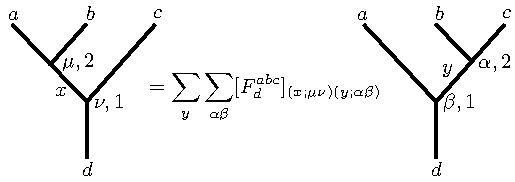
\includegraphics[scale=1.1]{Fsymbol_defn.pdf}}}},\ee
%Made it look like other F-symbols (dave)
\begin{align}
 \label{graphical_Fmove} 
\FusionSpaceLeftOrdered =\sum_y \sum_{\sigma \rho}\left( F^{abc}_d \right)_{(x; \mu \nu)(y;\sigma \rho)}   \FusionSpaceRightOrdered
\end{align}
where the greek indices label particular fusion space basis vectors, with $\mu\in V^{ab}_x,\nu\in V^{xc}_d,\alpha\in V^{bc}_y,$ and $\beta\in V^{ay}_d$, 
and where the first sum is over $y\in \sob(\spc)$. 
We also stick with the left-to-right ordering convention for the $F^{abcd}$ move:
%\dave{Changed order and and $x \ra x^*$.}
\be  
	F^{abcd} : \bigoplus_{x\in \sob(\spc)} V^{abx} \tp_{\End(x)} V^{x^*cd}   \;\to\;   \bigoplus_{y\in \sob(\spc)} V^{ayd} \tp_{\End(x)} V^{y^*bc} .
\ee
Which written as a matrix equation is
\ethan{The koszul order on the left diagram should be switched to match how we've written the $F$-move above}
\dave{done.}
\begin{align}
\label{PitchforkFMove}
\PitchforkFLeftprime = \sum_{y} \sum_{\rho \sigma} \left( F^{abcd} \right)_{(x; \mu \nu)(y; \rho \sigma)} \PitchforkFRightprime .
\end{align}

%\kw{$V^{y^*bc}$ here, but $V^{bcy^*}$ in the previous subsection; we should make this consistent (and also consistent with hamiltonian section}
%\dave{Ok, I'll change the other diagram since this is the definition of $F$ I used for the plaquette term in the Hamiltonian section.}
%\dave{I will fix this.}
%\dave{This has been fixed.}
We will also find the following identity helpful:
\begin{align}
\label{idpitchfork}
\Idabba = \sum_{x} \frac{d_x}{\mcb(\mu^* \tp \mu )} \IdPitchfork, 
\end{align}
where the pairing $\mcb$ is defined in \eqref{reflection_pairing_defn}.

%\kw{The K ordering used here has to be coordinated wsith the K ordering used in the definition of $B$.
%I think currently it is wrong, but the proposed change in the defn of $B$ \ethan{which $B$? $\mcb$?} will fix it.}
%\dave{I will fix this, and leave comment for KW and EL to check. }
%\ethan{right, the $\mu^*$ should be on the left. Left-to-right koszul ordering is correct though, right?}
%\dave{I changed $\mcb(\mu \tp \mu^*)$ to $\mcb(\mu^* \tp \mu)$ (to match new definition of pairing).}



%%%%%%%%%%%%%%%%%%
\subsection{Coherence relations} \label{coherence_ss}
%%%%%%%%%%%%%%%%%%

We will not list all coherence relations here.
Instead we will give a few examples, in order to highlight how the bosonic case
must be changed to take account of Koszul signs and relative tensor products.

\medskip

We will start with the well-known pentagon equation, in the version that uses the basic fusion spaces $V^{ab}_c$.
If we work in terms of {\it unordered maps}, with \eqref{fdef21} interpreted as an unordered map between direct sums of
unordered tensor products, then the fermionic pentagon equation looks just like the bosonic case, namely
that the following diagram commutes:
\begin{align}
\newcommand{\A}{\bigoplus_{p,q}V^{xy}_{p}\tp_p V^{pz}_{q}  \tp_q V^{qw}_{u}}
\newcommand{\AB}{\ar[rrrru]^{F^{pzw}_u} \ar[rrd]^{F^{xyz}_q}}
\newcommand{\B}{\bigoplus_{p,t} V^{xy}_{p} \tp_p V^{pt}_{u} \tp_t V^{zw}_{t}}
\newcommand{\BC}{\ar[rrrrd]^{F^{xyt}_u}}
\newcommand{\D}{\bigoplus_{r,q}V^{xr}_{q}\tp_r V^{yz}_{r}  \tp_q V^{qw}_{u}}
\newcommand{\DE}{\ar[rrrr]^{F^{xrw}_u} }
\newcommand{\E}{\bigoplus_{s,r}V^{xs}_{u}\tp_s V^{yz}_{r}  \tp_r V^{rw}_{s}}
\newcommand{\EF}{\ar[rru]^{F^{yzw}_s}} 
\newcommand{\F}{\bigoplus_{t,s} V^{xs}_{u} \tp_s V^{yt}_{s} \tp_t V^{zw}_{t}}
\vcenter{\xymatrix @!0 @M=5mm @R=28mm @C=16mm{
&&&&\B\BC&&&&\\
\A\AB&&&&&&&&\F\\
&&\D\DE&&&&\E\EF&&
	}} 
		\label{bosonPentagon}
\end{align}
%\dave{Formatting.}
\begin{comment} 
\begin{align}
\newcommand{\A}{\bigoplus_{p,q}V^{xy}_{p}\tp_p V^{pz}_{q}  \tp_q V^{qw}_{u}}
\newcommand{\AB}{\ar[rrru]^{F^{pzw}_u} \ar[rrd]^{F^{xyz}_q}}
\newcommand{\B}{\bigoplus_{p,t} V^{xy}_{p} \tp_p V^{pt}_{u} \tp_t V^{zw}_{t}}
\newcommand{\BC}{\ar[rrrrd]^{F^{xyt}_u}}
\newcommand{\D}{\bigoplus_{r,q}V^{xr}_{q}\tp_r V^{yz}_{r}  \tp_q V^{qw}_{u}}
\newcommand{\DE}{\ar[rrr]^{F^{xrw}_u} }
\newcommand{\E}{\bigoplus_{s,r}V^{xs}_{u}\tp_s V^{yz}_{r}  \tp_r V^{rw}_{s}}
\newcommand{\EF}{\ar[rru]^{F^{yzw}_s}} 
\newcommand{\F}{\bigoplus_{t,s} V^{xs}_{u} \tp_s V^{yt}_{s} \tp_t V^{zw}_{t}}
\vcenter{\xymatrix @!0 @M=2mm @R=22mm @C=19mm{
&&&\B\BC&&&&\\
\A\AB&&&&&&&\F\\
&&\D\DE&&&\E\EF&&
	}} 
	\label{bosonPentagon}
\end{align}
\end{comment}
where all the sums are over a representative set of simple objects and we have used the notation $\tp_x \equiv \tp_{\text{End}(x)}$.
%Technically, the modified tensor products $\tp_x$ also appear in the conventional bosonic pentagon equation, although in that 
%case we can set $\tp_x = \tp_\cc$ without loss of generality. 

However, if we peer under the hood and look at {\it ordered representatives} (as we would need to do if, for example,
we were checking the pentagon equation on a computer), then we
see that a Koszul sign appears:

\begin{comment} %version with explicit ordering
\begin{align}
\newcommand{\A}{\bigoplus_{p,q}V^{xy}_{p,3}\tp_p V^{pz}_{q,2}  \tp_q V^{qw}_{u,1}}
\newcommand{\AB}{\ar[rru]^{F^{pzw}_u} \ar[rrd]^{F^{xyz}_q}}
\newcommand{\B}{\bigoplus_{p,t} V^{xy}_{p,3} \tp_p V^{pt}_{u,1} \tp_t V^{zw}_{t,2}}
\newcommand{\BC}{\ar[rrr]^{F^{xyt}_u}}
\newcommand{\C}{\bigoplus_{t,s} V^{xs}_{u,1} \tp_s V^{yt}_{s,3} \tp_t V^{zw}_{t,2}}
\newcommand{\CF}{\ar[rrd]^{K_{23}}}
\newcommand{\D}{\bigoplus_{r,q}V^{xr}_{q,2}\tp_r V^{yz}_{r,3}  \tp_q V^{qw}_{u,1}}
\newcommand{\DE}{\ar[rrr]^{F^{xrw}_u} }
\newcommand{\E}{\bigoplus_{s,r}V^{xs}_{u,1}\tp_s V^{yz}_{r,3}  \tp_r V^{rw}_{s,2}}
\newcommand{\EF}{\ar[rru]^{F^{yzw}_s}} 
\newcommand{\F}{\bigoplus_{t,s} V^{xs}_{u,1} \tp_s V^{yt}_{s,2} \tp_t V^{zw}_{t,3}}
\vcenter{\xymatrix @!0 @M=2mm @R=22mm @C=19mm{
&&\B \BC &&&\C \CF &&\\
\A \AB &&&&&&&\F \\
&&\D \DE&&&\E \EF&&
	}} 
	\label{endoPentagon}
\end{align}
\end{comment}

%\kw{I propose we switch to this diagram}
%\dave{That's fine with me.}
%\kw{tentative to do: convert above diagram to left-to-right ordering}
\begin{align}
\newcommand{\A}{\bigoplus_{p,q}\Penta}
\newcommand{\AB}{\ar[rru]^{F^{pzw}_u} \ar[rrd]^{F^{xyz}_q}}
\newcommand{\B}{\bigoplus_{p,t} \Pentb}
\newcommand{\BC}{\ar[rrr]^{K_{23}}}
\newcommand{\C}{\bigoplus_{p,t} \Pentc}
\newcommand{\CF}{\ar[rrd]^{F^{xyt}_u}}
\newcommand{\D}{\bigoplus_{r,q}\Pentf}
\newcommand{\DE}{\ar[rrr]^{F^{xrw}_u} }
\newcommand{\E}{\bigoplus_{s,r}\Pente}
\newcommand{\EF}{\ar[rru]^{F^{yzw}_s}} 
\newcommand{\F}{\bigoplus_{t,s} \Pentd}
\vcenter{\xymatrix @!0 @M=2mm @R=28mm @C=19mm{
&&\B \BC &&&\C \CF &&\\
\A \AB &&&&&&&\F \\
&&\D \DE&&&\E \EF&&
	}} 
	\label{endoPentagonDiagram}
\end{align}
or equivalently, 
\begin{align}
\newcommand{\A}{\bigoplus_{p,q}V^{qw}_{u}\tp_q V^{pz}_{q}  \tp_p V^{xy}_{p}}
\newcommand{\AB}{\ar[rru]^{F^{pzw}_u} \ar[rrd]^{F^{xyz}_q}}
\newcommand{\B}{\bigoplus_{p,t} (V^{pt}_{u} \tp_t V^{zw}_{t}) \tp_p V^{xy}_{p}}
\newcommand{\BC}{\ar[rrr]^{K_{23}}}
\newcommand{\C}{\bigoplus_{p,t} (V^{pt}_{u} \tp_p V^{xy}_{p}) \tp_t V^{zw}_{t}}
\newcommand{\CF}{\ar[rrd]^{F^{xyt}_u}}
\newcommand{\D}{\bigoplus_{r,q}V^{qw}_{u}\tp_q V^{xr}_{q}  \tp_r V^{yz}_{r}}
\newcommand{\DE}{\ar[rrr]^{F^{xrw}_u} }
\newcommand{\E}{\bigoplus_{s,r}V^{xs}_{u}\tp_s V^{rw}_{s}  \tp_r V^{yz}_{r}}
\newcommand{\EF}{\ar[rru]^{F^{yzw}_s}} 
\newcommand{\F}{\bigoplus_{t,s} V^{xs}_{u} \tp_s V^{yt}_{s} \tp_t V^{zw}_{t}}
\vcenter{\xymatrix @!0 @M=2mm @R=22mm @C=19mm{
&&\B \BC &&&\C \CF &&\\
\A \AB &&&&&&&\F \\
&&\D \DE&&&\E \EF&&
	}} 
	\label{endoPentagon}
\end{align}
Here, $K_{23}$ denotes the Koszul isomorphism associated to transposing the second and third tensor factors.
Again, we are using the implicit left-to-right Koszul ordering of each tensor product.
In terms of the matrix elements of the $F$-symbols, this reads 
\be  
\begin{aligned}
 \sum_{r\in \sob(\spc)}
 \sum_{\sigma\in V^{xr}_q}
 \sum_{\omega \in V^{yz}_r}
 \sum_{\eta\in V^{rw}_s}
 & 
 [F^{xyz}_q]_{(p;\mu\nu)(r;\omega\sigma)}
 [F^{xrw}_u]_{(q;\sigma\lambda)(s;\eta\gamma)}
 [F^{yzw}_s]_{(r;\omega \eta)(t;\alpha\delta)} \\ 
 & = \sum_{\beta \in V^{pt}_u}
 [F^{pzw}_u]_{(q;\nu\lambda)(t;\alpha\beta)}
 (-1)^{|\mu||\alpha|}
 [F^{xyt}_u]_{(p;\mu\beta)(s;\delta \gamma)}, 
\end{aligned} 
\ee
where $\mu\in V^{xy}_p,\nu\in V^{pz}_q,\lambda\in V^{qw}_u,\gamma\in V^{xs}_u,\delta\in V^{yt}_s,$ and $\alpha\in V^{zw}_t$. 
The Koszul sign $K_{23}$ appearing in \eqref{endoPentagon} appears in the above formula as $(-1)^{|\mu||\alpha|}$. 
%\dave{I found:
% $\beta$ in 3rd F-symbol, first line should be $\omega$.
%The subscript $p$ in the first F-symbol of the second line should be $q$
%}
%\ethan{thanks, they were typos}

%The Koszul ordering of each tensor product in the diagram is obtained with the help of the conventions in 
%\eqref{Fmove_ordering_conventions}. 
%In terms of the matrix elements of the $F$-symbols, this reads 
%\be  \begin{aligned} \sum_{r\in {\rm sObj}(\spc)}\sum_{\sigma\in V^{xr}_q}\sum_{\omega \in V^{yz}_r}\sum_{\eta\in V^{rw}_s}& [F^{xyz}_q]_{(p;\mu\nu)(r;\omega\sigma)}[F^{xrw}_u]_{(q;\sigma\lambda)(s;\eta\gamma)}[F^{yzw}_s]_{(r;\beta\eta)(t;\alpha\delta)} \\ & = \sum_{\beta \in V^{pt}_u}(-1)^{|\delta||\alpha|}[F^{pzw}_u]_{(p;\nu\lambda)(t;\alpha\beta)}[F^{xyt}_u]_{(p;\mu\beta)(s;\delta\gamma)}, \end{aligned} \ee

%where $\mu\in V^{xy}_p,\nu\in V^{pz}_q,\lambda\in V^{qw}_u,\gamma\in V^{xs}_u,\delta\in V^{yt}_s,$ and $\alpha\in V^{zw}_t$. 
%The Koszul sign $P_{23}$ appearing in \eqref{endoPentagon} appears in the above formula as $(-1)^{|\delta||\alpha|}$. 

%\dave{I think we should draw this one in the pitch fork basis. 
%I can do that.}
Other coherence relations are modified to take into account Koszul 
signs.
For example, requiring consistency between $F$-moves and the pivot means that the following 
diagram must commute:
%\dave{I will delete these comments, change $P_{12}$ to $K_{12}$ in picture, and also $P$ to $P^{-1}$ on RHS.}
%\dave{Would we prefer to define the pivot in \eqref{Pitchfork_pivot} to keep the outer legs fixed and rotate the inner pitchfork, 
%so that it maps between the same vector space (as I did in the following). 
%Or would we prefer to leave it as a map between different vector spaces?
%For coherence conditions like the following I think the first is simpler.
%}
%\ethan{agreed about just rotating the inner pitchfork. I like this better and I think it's what we had originally}
%\dave{Should we re-define it in the definition section or just add a footnote here describing what we mean?} 
%\ethan{I lean towards having it act on the same vector space everywhere in the paper. Kevin, do you have a preference?}
%\ethan{Although after talking with Dave, I think we came to the conclusion that we should use both simultaneously} 
\dave{Changed Koszul ordering in definition of $F^{abcd}$, and modified this equation correspondingly.}
\ethan{Looks good now}
\begin{align}
\newcommand{\A}{\bigoplus_x \PitchforkFLeftprimesmall}
\newcommand{\B}{\bigoplus_x  \PivotCoherenceb}
\newcommand{\C}{\bigoplus_x\;  \PivotCoherencec  }
\newcommand{\D}{\bigoplus_y   \PivotCoherencea }
\newcommand{\E}{\bigoplus_y \PitchforkFRightprimesmall }
\vcenter{\xymatrix @!0 @M=1.5mm @R=25mm @C=30mm{
&\A  \ar[rr]^{F^{abcd}} &&\E \ar[rd]^{(P^{ayd})^{-1}}&\\
\B\ar[ru]^{K_{12}} &&&&\D \ar[lld]^{F^{dabc}}   \\
&&\C \ar[llu]^{P^{dxc} \tp P^{x^*ab} } &&
	}} 
	\label{pivotconsistent}
\end{align} 


\begin{comment} %non-diagrammatic notation
\begin{align}
\newcommand{\A}{\bigoplus_x V^{ab}_{x,2} \tp_x V^{xc}_{d,1}}
\newcommand{\B}{\bigoplus_y V^{ay}_{d,1} \tp_y V^{bc}_{y,2} }
\newcommand{\C}{\bigoplus_y V^{dd^*} \tp_{d^*} V^{d^* a}_{y,1} \tp_y V^{yb}_{c^*,2}  \tp_{c^*} V_{c^*c}  }
\newcommand{\D}{\bigoplus_x V^{dd^*} \tp_{d^*} V^{d^*x}_{c^*,2} \tp_x V^{ab}_{x,1}  \tp_{c^*} V_{c^*c} }
\newcommand{\E}{\bigoplus_x V^{ab}_{x,1} \tp_x V^{xc}_{d,2}}
\vcenter{\xymatrix @!0 @M=4mm @R=25mm @C=30mm{
&\A \ar[ld]^{F^{abc}_d}\ar[rr]^{K_{12}} &&\E&\\
\B \ar[rd]^{P^{ay}_{d,1} \tp K^{bc}_{y,2} \circ (\kappa_d  \kappa_y \kappa_c)^{-1}}&&&&\D \ar[ul]^{\kappa_d \kappa_c \circ (P^{d^*x}_{c^*,2})^{-1}} \\
&&\C &\ar[ru]^{F^{d^*ab}_{c^*}}&
	}} 
	\label{pivotconsistent}
\end{align} 
\end{comment}


%%%%%%%%%%%%%%%%%%
\subsection{Reflection structure} \label{reflection_ss}
%%%%%%%%%%%%%%%%%%

A {\it reflection structure} on $\spc$ is an antilinear anti-automorphism $r$ from $\spc$ to itself which preserves (rather than reverses) 
the the tensor product:
\begin{align}
	a & \; \mapsto \; r(a) \\
	\alpha: a\to b & \; \mapsto \; r(\alpha): r(b) \to r(a) \\
	r(\lambda \alpha) & \;=\;  \bar\lambda r(\alpha) \\
	r(a\tp b) & \;=\;  r(a) \tp r(b) \\
	r(\alpha\tp \beta) & \;=\;  r(\alpha) \tp r(\beta)
\end{align}
for objects $a,b$ and morphisms $\alpha,\beta$. \ethan{added the following to make things a little more friendly:} Diagrammatically, the action of  $r$ 
reflects diagrams about the horizontal axis (while acting as complex conjugation on $\cc$). 
Outside of this section, we usually denote $r$ by a bar: $\bar a = r(a)$ and $\bar\alpha = r(\alpha)$.

For objects, we require that $r(r(a)) = a$.
\ethan{Seems like we also require $r(a)=a$ for a good deal of the paper?}
For morphisms, we have two choices.
In a pin+ reflection structure, we require $r^2$ to be the identity functor:
\be
	r^2 = \id .
\ee
In a pin$-$ reflection structure, we require $r^2$ to be the spin flip functor,
\be
	r^2 = (-1)^F .
\ee
The main examples of this paper all have pin+ reflection structures.

We require $r$ to be compatible with the other structure maps of $\spc$ (pivots, $F$, etc.).
For example, %\kw{see pdf notes for examples}
we require the following diagrams to be commutative:
\begin{align}
\vcenter{
\xymatrix @!0 @M=2mm @R=34mm @C=19mm{
\refa \ar[rr]^r \ar[d]_P&& \refb\\
\refd \ar[rr]^r&&\refc \ar[u]^P\\
	}}
\end{align}
and
\begin{align}
\vcenter{
\xymatrix @!0 @M=2mm @R=34mm @C=19mm{
\refcoha\ar[rr]^{F^{abc}_d} \ar[d]_r &&\refcohb \ar[rr]^r && \refcohc \ar[d]^{P_L^{-1} \tp P_R} \\
\refcohh\ar[rr]^{P_R \tp P_L^{-1}} &&\refcohg \ar[d]_{K_{12}} && \refcohd \ar[d]^{K_{12}} \\
    &&\refcohf && \refcohe \ar[ll]^{F^{\bar{a}^* \bar{d} \bar{c}^*}_{\bar{b}}} \\
	}}
\end{align}

A pin+ reflection structure on $\spc$ allows us to define the action of pin+ diffeomorphisms on $\spc$ string nets.

It follows from the ``back wall" line bundle construction of Appendix \ref{flb_appendix} that super pivotal categories $\mcc/\psi$
obtained via fermion condensation will have pin+ reflection structures whenever the parent category has an
ordinary bosonic reflection structure.
\kw{should make sure we believe this; maybe add remark to appendix}
\ethan{agreed}

Our main use for pin+ reflections is to define a sesquilinear inner product on the string net space $A(Y; c)$.
Let $Y$ be a spin surface and let $-Y$ denote the same underlying surface but with the reversed spin structure.
The ``identity" map from $Y$ to $-Y$ is not a spin diffeomorphism (as it reverses orientation), but it is a pin+ diffeomorphism.
Using the reflection structure on $\spc$, we can use this pin+ diffeomorphism to map string nets in $A(Y; c)$ to 
string nets in $A(-Y; r(c))$.
If $r(c) = c^*$, then string nets in $A(Y;c)$ and $A(-Y;r(c))$ can be glued together to get a string net on the closed
spin surface $Y\cup_{\bd Y} -Y = \bd(Y\times I)$.
Using the path integral $Z(Y\times I) : A(Y\cup_{\bd Y} -Y) \to \cc$ now yields a sesquilinear inner product on $A(Y;c)$.
Since $A(Y;c)$ is finite-dimensional, we also get an inner product on the dual space $Z(Y;c)$.

Let $M$ be a spin 3-manifold.
Then the path integrals $Z(M): A(\bd M)\to \cc$ and $Z(-M): A(-\bd M)\to \cc$ are related by
\be \label{3man-pi-orev}
	Z(-M) = Z(M)\circ R ,
\ee
where $R:A(-\bd M) \to A(\bd M)$ is the antilinear map induced by the orientation-reversing identity map from $-\bd M$ to $\bd M$.
Equivalently, $Z(M)\in Z(\bd M)$ and $Z(-M)\in Z(- \bd M)$ and
\be \label{3man-pi-orevz}
	Z(M) = R(Z(-M)) .
\ee

Let $Y_1$ and $Y_2$ be spin surfaces and let $M$ be a cobordism from $Y_1$ to $Y_2$
(i.e.\ $\bd M = Y_2\cup -Y_1$).
Then $-M$ is a cobordism from $Y_2$ to $Y_1$.
The path integrals can be viewed as maps $Z(M): Z(Y_1)\to Z(Y_2)$ and $Z(-M):Z(Y_2)\to Z(Y_1)$.
It follows from \eqref{3man-pi-orevz} that $Z(-M)$ is the adjoint of $Z(M)$ with respect to the inner products on $Z(Y_1)$
and $Z(Y_2)$ defined above.
%\kw{It will take more work to show that the hamiltonians of sec 9 are Hermitian; if we do that work it should probably
%go in sec 9}
%\ethan{As discussed I think we should punt, adding something like ``The hamiltonian can be show to be hermitian using the techniques discussed in ref(reflection)'' to the Hamiltonian section.}





%\bigskip
%
%\kw{TO DO: discuss reflection structures, pin, etc.
%probably just give basic defs}
%\ethan{Are we wanting to talk about inner products and stuff? I think we can largely just refer to stuff in the line bundle appendix}
%\dave{Should probably say at least enough so that we know the Hamiltonian is hermitian.}



%%%%%%%%%%%%%%%%
%%%%%%%%%%%%%%%%
%%%%%%%%%%%%%%%%
\begin{comment}

%what follows until the next triple-line of %'s is old stuff, which is essentially a more verbose version of what we've kept above
%%%%%%%%%%%%%%%%%%%%%%%%%%%%%%%%%%%%%%%
\subsection{Modified tensor product (old version)}
%%%%%%%%%%%%%%%%%%%%%%%%%%%%%%%%%%%%%%%

\kw{I think this section can be shortened; I think some of the material already appears far above.}

There is an important subtlety involved when we tensor together fusion spaces which involve q-type particles, which stems from the non-triviality of the fusion space $V^{x\unit}_x$ if $x$ is q-type.
To see where this comes from, suppose $x$ is a q-type particle, and consider the resolution of the identity 
\begin{align} \label{resid}
\Hom(x,x) \cong \bigoplus_y \Hom(x,y) \tp_\cc \Hom(y,x),
\end{align}
where $x$ is any object and the sum runs over simple objects $y$. 
The above relation is actually {\it incorrect} when q-type particles are involved. 
Indeed, if $x$ is simple then \eqref{resid} reads $\Hom(x,x) = \Hom(x,x) \tp_\cc \Hom(x,x).$ 
If $x$ is q-type then $\End(x) = \cliff_1$ implies $\cliff_1 \cong \cliff_1\tp_\cc \cliff_1 \cong \cliff_2$, which is a contradiction. 
Furthermore, if $x$ is q-type then by iterating we see that the supervector space associated with a vertical $x$ worldline is $\End(x)^{\tp_{\cc} n} \cong \cliff_n$ for arbitrarily large $n$, the dimension of which can be made arbitrarily large by increasing $n$. 
Alternatively, we can also observe that the product $V_{\unit,1}^{xx} \tp_\cc V^\unit_{xx,2} \tp_\cc \dots \tp_\cc V_{\unit,n-1}^{xx} \tp_\cc V^\unit_{xx,n}$ is both isotopy-equivalent to $V^{x\unit}_x \cong \cliff_1$ and isomorphic to $\cliff_n$, which is also a contradiction. 
These results mean that in the present formulation, the sizes of the Hilbert spaces assigned to fusion diagrams are not even well-defined! 

In order to fix these inconsistencies, we need to mod out by ``internal'' degrees of freedom carried by q-type particles when taking tensor products. 
These internal degrees of freedom are encapsulated in the fusion spaces $V^{x\unit}_x, V^{\unit x}_x,$ and $V^{xx}_\unit$, each of which is $\cliff_1$ if $x$ is q-type.
Graphically, modding out by these internal degrees of freedom is equivalent to modding out by local relations involving fermions and q-type particles.  
These relations are given by locally sliding fermions along a q-type edge from one fusion vertex to another.
A tensor product between fusion spaces taken over a q-type particle must be quotiented by ``sliding isomorphisms'' like this. 

To perform the modding out procedure described above, we examine the 
equivalence relation 
\begin{align} \label{equivreln}
(V^{ab}_{x,1} f_3) \tp_{\mathbb{C}}V^{xc}_{d,2} \sim V^{ab}_{x,1} \tp_{\mathbb{C}} (f_3 V^{xc}_{d,2})
\end{align}
where $f_3$ is an odd endomorphism of $x$ (as before, the numerical subscripts keep track of the Koszul ordering).
This equivalence relation establishes an equivalence between states that differ by the placement of {\it odd} elements between factors in a tensor product involving q-type particles. 
Since $\cliff_1 = \langle1,f\rangle$ and $\End(x) = \cliff_1$ if $x$ is q-type, this can be accomplished by using $\End(x)$ as the tensor unit, {\it instead} of $\cc$. 
This means that in order to achieve a self-consistent fermionic theory, we need to replace the tensor product of two fusion spaces linked by the simple object $x$ with a tensor product over $\End(x)$. 
 Explicitly, to construct a fermionic theory, we must make the following replacements:
\be \ba
 &V^{ab}_{x,2} \tp_{\mathbb{C}} V^{xc}_{d,1}\quad  \text{is replaced by} \quad V^{ab}_{x,2} \tp_{\text{End}(x)} V^{xc}_{d,1},\ \  {\rm and} \\ 
  &V^{ax}_{d,1} \tp_{\mathbb{C}} V^{bc}_{x,2}\quad  \text{is replaced by} \quad V^{ax}_{d,1} \tp_{\End(x)} V^{bc}_{x,2},
\ea 
\ee
where $\tp_{\End(x)}$ means that $\End(x)$ is taken to be the tensor unit. Explicitly, 
\begin{align}
V^{ab}_{x,1} \tp_{\text{End}(x)} V^{xc}_{d,2} = V^{ab}_{x,1} \tp_{\mathbb{C}}V^{xc}_{d,2}/ \sim,
\label{qtensor}
\end{align}
where $\sim$ is the equivalence relation \eqref{equivreln}. 
Analogous relations hold for fusion spaces connected in different ways. 

Using the modified tensor product allows us to easily write down the correct version of \eqref{resid}, which is 
\begin{align}
\Hom(x,x) \cong \bigoplus_y \Hom(x,y) \tp_{\End(y)} \Hom(y,x).
\end{align}
In particular, if $x$ is a simple q-type object, then we (correctly) have \be
\cliff_1 \cong \Hom(x,x) \cong \Hom(x,x)\tp_{\End(x)} \Hom(x,x) \cong \cliff_1\tp_{\cliff_1}\cliff_1 \cong \cliff_1.\ee  

To take the modified tensor product $\End(x)$ when doing calculations or solving consistency equations numerically, we find it easiest to directly impose the condition that physical vectors in the space $V^{ab}_x \tp_{\mathbb{C}} V^{xc}_d$ be left invariant under the action of $\text{End}(x)$. 
There are two types of fusion diagrams we need to consider, depending how the fusion vertices that they are formed from are connected. This leads to two isomorphisms of fusion diagrams:
\begin{align}
&\vcenter{\xymatrix @!0 @M=1mm @C=42mm{
 &L_f: \; \;V^{ab}_{x,2} \tp_{\mathbb{C}} V^{xc}_{d,1} \ar[r]            & V^{ab}_{x,2} \tp_{\mathbb{C}} V^{xc}_{d,1}  \\
		  &\;\;\;\;\;\;\; \ket{\psi}\tp_\mathbb{C} \ket{\eta}  \ar@{|->}[r] & (f\ket{\psi}) \tp_{\mathbb{C}} (f^{-1} \ket{\eta})  
		  }} \quad \quad f \in \text{End}(x)\\
		  \\		  
&		  \vcenter{\xymatrix @!0 @M=1mm @C=42mm{
		  &R_f: \; \;V^{ay}_{d,1} \tp_{\mathbb{C}} V^{bc}_{y,2} \ar[r]            & V^{ay}_{d,1} \tp_{\mathbb{C}} V^{bc}_{y,2} \\
		  &\;\;\;\;\;\;\; \ket{\psi}\tp_\mathbb{C} \ket{\eta}  \ar@{|->}[r] & (f\ket{\psi}) \tp_{\mathbb{C}} (f^{-1} \ket{\eta})
	}}	\quad \quad f \in \text{End}(y)
	\label{DotSlide}
	\end{align}
We note that both $L_f$ and $R_f$ are always {\it even} maps, regardless of the parity of $f$. 

Tensoring over endomorphisms in a fusion space is equivalent to requiring the fusion space to be invariant under the action of $L_f$ and $R_f$. 
Said another way, any vectors related by application of $L_f$ or $R_f$ are considered equivalent, which makes it natural to think of $L_f$ and $R_f$ as gauge transformations, since they encode redundancy in physical vector spaces.

It is often useful to do calculations 
by working with explicit choices of representatives of vectors in each isomorphism class, imposing the requirement that any diagrammatic manipulation commutes with all endomorphisms generated by $L_f$ and $R_f$. 
After doing calculations, we can project back onto the physical subspace by modding out by the equivalence relation \eqref{equivreln}. 
This can be done provided that $L_f$ and $R_f$ commute on any fusion diagram. For example, for a fusion diagram built from three fusion vertices, we require that
\begin{align}
L_{f, 32}L_{g,21} V^{ab}_{x,3} \tp_{\mathbb{C}} V^{xc}_{y,2} \tp_{\mathbb{C}} V^{yd}_{w,1} = L_{g,21} L_{f, 32} V^{ab}_{x,3} \tp_{\mathbb{C}} V^{xc}_{y,2} \tp_{\mathbb{C}} V^{yd}_{w,1} 
\end{align}
for all $f \in \text{End}(x)$ and $g \in \text{End}(y)$. 
From now, when we write $\tp$ we will always mean $\tp_\cc$, unless specified otherwise.




As alluded to earlier, quotienting by the local relations like \eqref{equivreln} is reminiscent of the 
condensation of electron pairs in superconductors: these relations say that pairs of fermions can be freely 
added or removed from the condensate, and that fermions lines terminating on q-type objects (which are 
the Majorana spin structure defects in this analogy) are able to move around freely. 
Indeed, a fermionic phase of matter will generate such terms at second order in perturbation theory when 
proximity coupled to a superconductor.
Thus, heuristically, we can think of q-type particles as the result of proximity induced superconductivity on 
a fusion category with only m-type particles.


%%%%%%%%%%%%%%%%%%
\subsection{F-symbols (old version)}
%%%%%%%%%%%%%%%%%%

The $F$-symbols are defined as basis transformations between different fusion spaces. 
There are two additional considerations when defining the $F$-symbols in the fermionic setting: they must account for the normal-ordering of the fusion spaces that are transformed during the $F$-move, and they must incorporate the modified tensor product introduced in Section \ref{modified_tensor_product}. 

There is some arbitrariness involved in our definition of the $F$-moves. They must be linear 
transformations between two different fusion graphs with four outgoing anyon worldlines, although the 
details of the structure of the graphs they provide a relation between (e.g.\ how many of their outgoing legs 
point up or down) is arbitrary, with the different choices being related by pivotal matrices $P^{ab}_c$ which 
will be defined in the following section. 
Additionally, we must choose how they act on the relative sign-ordering of the fusion spaces involved in 
the $F$-move. We will choose the following convention (standard in the physics literature), in which the $F$-symbols are basis 
transformations between two fusion spaces of the form $V^{ab}_c$.
We will also choose a convention in which the vertical Koszul
of the fusion spaces in any diagram is preserved under $F$-moves: 
\begin{align} \label{Fdef}
F^{abc}_d: \; \; \bigoplus_x V^{ab}_{x,2} \tp_{\text{End}(x)} V^{xc}_{d,1} \rightarrow \bigoplus_y V^{ay}_{d,1} \tp_{\text{End}(y)} V^{bc}_{y,2}
\end{align}
Graphically, this is written in terms of the matrix elements of $F$ as
\be \label{graphical_Fmove} \mathord{\vcenter{\hbox{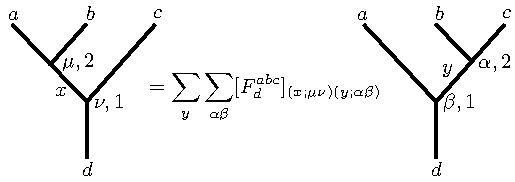
\includegraphics[scale=1.1]{Fsymbol_defn.pdf}}}},\ee
where the greek indices label particular fusion space basis vectors, with $\mu\in V^{ab}_x,\nu\in V^{xc}_d,\alpha\in V^{bc}_y,$ and $\beta\in V^{ay}_d$.
When we take tensor products of fusion spaces, the fusion spaces appear in the tensor product in the 
same left-to-right order that they appear in the fusion diagram, while the Koszul ordering of the fusion 
spaces to increase as we go ``up'' the diagram. 
This means that the $F$-move permutes the normal ordering of the fusion spaces appearing in the fusion 
diagram, which we will see leads to Koszul-sign modifications of the pentagon relation. 

We stress that the multiplicity indices $\mu,\nu,$ etc. appearing in \eqref{graphical_Fmove} account 
for both regular degeneracies in fusion spaces (as is present in bosonic theories), as well as for 
the parity of the fusion spaces. This means that in fermionic theories, the $\mu$ indices will generically 
run over both even and odd vectors. For example, if one of $a,b,c$ is q-type, then $V^{ab}_c$ is acted 
on naturally by $\cliff_1$, and so is of the form $V^{ab}_c\cong \cc^{n|n}$, meaning that a sum over $\mu\in V^{ab}_c$
contains $2n$ different summands.  

To implement the modified tensor products $\tp_{\End(x)}$ and $\tp_{\End(y)}$ in \eqref{Fdef}, we impose 
the condition that the F-symbols commute with the gauge transformations $L,R$ that implement the 
modified tensor product. 
Imposing this condition means that the following diagram must commute:
\begin{align}
	\vcenter{\xymatrix @!0 @M=1mm @R=30mm @C=42mm{
		 \bigoplus_x V^{ab}_{x,2} \otimes V^{xc}_{d,1} \ar[d]^{L_{f}}\ar[r]^{F^{abc}_d}& \bigoplus_y V^{ay}_{d,1} \otimes V^{bc}_{y,2} \ar[d]^{R_{g}} \\
		\bigoplus_x V^{ab}_{x,2} \otimes V^{xc}_{d,1}  \ar[r]^{F^{abc}_d}  & \bigoplus_y V^{ay}_{d,1} \otimes V^{bc}_{y,2}	
	}} 
	{ \quad\quad \forall f \in \oplus_x \text{End}(x), \; \; g \in \oplus_y \text{End}(y)}
	\label{Fcommute}
\end{align}
In matrix form, this is simply $F^{abc}_d  L_f=   R_g F^{abc}_d$.

The pentagon relation in the superfusion case is defined as an equivalence between the same two diagrammatic manipulations as in the bosonic case, and is the statement that the following diagram commutes:
\begin{align}
\newcommand{\A}{\bigoplus_{p,q}V^{xy}_{p,3}\tp_p V^{pz}_{q,2}  \tp_q V^{qw}_{u,1}}
\newcommand{\AB}{\ar[rru]^{F^{pzw}_u} \ar[rrd]^{F^{xyz}_q}}
\newcommand{\B}{\bigoplus_{p,t} V^{xy}_{p,3} \tp_p V^{pt}_{u,1} \tp_t V^{zw}_{t,2}}
\newcommand{\BC}{\ar[rrr]^{F^{xyt}_u}}
\newcommand{\C}{\bigoplus_{t,s} V^{xs}_{u,1} \tp_s V^{yt}_{s,3} \tp_t V^{zw}_{t,2}}
\newcommand{\CF}{\ar[rrd]^{P_{23}}}
\newcommand{\D}{\bigoplus_{r,q}V^{xr}_{q,2}\tp_r V^{yz}_{r,3}  \tp_q V^{qw}_{u,1}}
\newcommand{\DE}{\ar[rrr]^{F^{xrw}_u} }
\newcommand{\E}{\bigoplus_{s,r}V^{xs}_{u,1}\tp_s V^{yz}_{r,3}  \tp_r V^{rw}_{s,2}}
\newcommand{\EF}{\ar[rru]^{F^{yzw}_s}} 
\newcommand{\F}{\bigoplus_{t,s} V^{xs}_{u,1} \tp_s V^{yt}_{s,2} \tp_t V^{zw}_{t,3}}
\vcenter{\xymatrix @!0 @M=2mm @R=22mm @C=19mm{
&&\B \BC &&&\C \CF &&\\
\A \AB &&&&&&&\F \\
&&\D \DE&&&\E \EF&&
	}} 
	\label{endoPentagon}
\end{align}
where we have used the notation $\tp_x \equiv \tp_{\text{End}(x)}$. Note that this is actually a hexagon, 
not a pentagon: the extra arrow is the one marked $P_{23}$, which is the Koszul sign originating from 
switching the Koszul ordering of the $V^{yt}_s$ and $V^{zw}_t$ fusion spaces. 

The use of the modified tensor products $\tp_x$ is how (\ref{endoPentagon}) differs from the ``super-
pentagon" equation which has already appeared in the literature \cite{Gu2015, gaiotto2016, usher2016} 
and which is only applicable to theories that possess no q-type objects 
(note that if our theory has no q-type objects we can set $\tp_x = \tp_\cc$ for all $x$, and so 
\eqref{endoPentagon} reduces to the super-pentagon equation in the case with no q-type particles).
In practice, it is often easiest to first solve the pentagon equation in the ``extended space'' by replacing all 
$\tp_x$ tensor products with $\tp_\cc$ (yielding the super pentagon equation), and then requiring the 
resulting $F$-symbols to satisfy the constraint (\ref{Fcommute}), which is tantamount to implementing the 
modified tensor products.

As a matrix equation, the pentagon relation \eqref{endoPentagon} reads 
\be  \begin{aligned} \sum_{r\in {\rm sObj}(\mcc)}\sum_{\sigma\in V^{xr}_q}\sum_{\omega \in V^{yz}_r}\sum_{\eta\in V^{rw}_s}& [F^{xyz}_q]_{(p;\mu\nu)(r;\omega\sigma)}[F^{xrw}_u]_{(q;\sigma\lambda)(s;\eta\gamma)}[F^{yzw}_s]_{(r;\beta\eta)(t;\alpha\delta)} \\ & = \sum_{\beta \in V^{pt}_u}(-1)^{|\delta||\alpha|}[F^{pzw}_u]_{(p;\nu\lambda)(t;\alpha\beta)}[F^{xyt}_u]_{(P;\mu\beta)(s;\delta\gamma)}, \end{aligned} \ee
where $\mu\in V^{xy}_p,\nu\in V^{pz}_q,\lambda\in V^{qw}_u,\gamma\in V^{xs}_u,\delta\in V^{yt}_s,$ and $\alpha\in V^{zw}_t$. 
The Koszul sign $P_{23}$ appearing in \eqref{endoPentagon} appears in the above formula as $(-1)^{|\delta||\alpha|}$, where as usual $|\delta|$ denotes the parity 
of the vector $\delta$. 


%%%%%%%%%%%%%%%%%%%%
\subsubsection{Pivotal structure (old version)}
%%%%%%%%%%%%%%%%%%%%

Finally, we remark on the pivotal structure of fusion spaces in superfusion categories. First, we have the Frobenius-Schur indicator, which is given by
\begin{align}
&\kappa_a: \;\; V^{a a^*} \tp_{\text{End}(a^*)} V_{a^*a} \rightarrow V^a_a
\end{align}
Diagrammatically, 
\be \mathord{\vcenter{\hbox{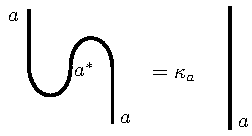
\includegraphics[scale=1]{FS_defn.pdf}}}}
 \ee
The Frobenius-Schur move is a special case of the pivot: 
\begin{align}
&P^{ab}_c: \; \; V^{c^* c} \tp_{\End(c)} V^{ab}_c \tp_{\End(b)} V_{b b^*} \rightarrow V^{c^* a}_{b^*} 
\end{align}
Diagrammatically, this looks like 
\be \mathord{\vcenter{\hbox{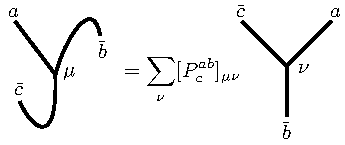
\includegraphics[scale=1.1]{pivot_defn.pdf}}}}
\ee
In terms of the pivot, we see that $\kappa_a = [P^{0a^*}_{a^*}]_{00}$. From the diagrammatics, we see that the pivot implements a $2\pi/3$ rotation of the fusion space. 
Acting with $P$ three times thus performs a $2\pi$ rotation of a fusion vertex:
\be \mathord{\vcenter{\hbox{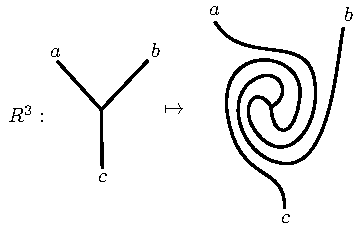
\includegraphics[scale=1]{pivot_cubed.pdf}}}}\ee
In bosonic theories, we must always have $P^3=\unit$: rotating a fusion vertex by $2\pi$ is equivalent to doing nothing.
In the superfusion setting there is a more interesting posibility, because acting with $P^3$ on some vector $v\in V^{ab}_c$ performs a $2\pi$ rotation on the fermion framing of $v$.
Rotating the fermion framing is equivalent to multiplication by $-1$ if $v$ has odd fermion parity. 

Therefore, in superfusion categories, the pivotal structure relation $P^3=\unit$ is realized {\it projectively}, in the sense that 
\be P^3 = (-1)^F \unit,\ee
where $(-1)^F$ is the fermion parity operator, which acts on any $v\in V^{abc}$ as $(-1)^F v = (-1)^{|v|}v$.

We now discuss the relationship between the $F$-symbols and the pivotal structure. 
The pivots can be obtained from the quantum dimensions and the $F$-symbols through 
\be [P^{ab}_c]_{\mu\nu} = \sum_\lambda d_b [F^{abb^*}_a]_{(c;\mu\lambda)(0;00)} [F^{c^* c b^*}_{b^*}]_{(0;00)(a;\lambda\nu)}.\ee
Additionally, consistency between the pivotal structure and $F$-moves requires that the following diagram commute: 
\begin{align}
\newcommand{\A}{\bigoplus_x V^{ab}_{x,2} \tp_x V^{xc}_{d,1}}
\newcommand{\B}{\bigoplus_y V^{ay}_{d,1} \tp_y V^{bc}_{y,2} }
\newcommand{\C}{\bigoplus_y V^{dd^*} \tp_{d^*} V^{d^* a}_{y,1} \tp_y V^{yb}_{c^*,2}  \tp_{c^*} V_{c^*c}  }
\newcommand{\D}{\bigoplus_x V^{dd^*} \tp_{d^*} V^{d^*x}_{c^*,2} \tp_x V^{ab}_{x,1}  \tp_{c^*} V_{c^*c} }
\newcommand{\E}{\bigoplus_x V^{ab}_{x,1} \tp_x V^{xc}_{d,2}}
\vcenter{\xymatrix @!0 @M=4mm @R=25mm @C=30mm{
&\A \ar[ld]^{F^{abc}_d}\ar[rr]^{P_{12}} &&\E&\\
\B \ar[rd]^{P^{ay}_{d,1} \tp P^{bc}_{y,2} \circ (\kappa_d  \kappa_y \kappa_c)^{-1}}&&&&\D \ar[ul]^{\kappa_d \kappa_c \circ (P^{d^*x}_{c^*,2})^{-1}} \\
&&\C &\ar[ru]^{F^{d^*ab}_{c^*}}&
	}} 
	\label{pivotconsistent}
\end{align} 

The final pivotal data we will need to employ concerns sliding fermions along q-type strings. 
Define 
\begin{align}
\TwodotCap =  \lambda_{\text{cap}} \; \Qcap \quad \quad
\TwodotCup =  \lambda_{\text{cup}}\; \Qcup \quad \quad
\Qdotdot =  \lambda \; \QIdentity,
\end{align}
where the black lines denote arbitrary string-net configurations on which the q-type strings terminate.
With these definitions one can show that
\begin{align}
\QCapDotL =(-\lambda_{\text{cap}}^{-1} \lambda )\; \QCapDotR \qquad \qquad \QCapDotR  = (\lambda_{\text{cap}}^{-1} \lambda ) \; \QCapDotL\\ 
\\
\QCupDotR= (-\lambda_{\text{cup}}^{-1} \lambda )\; \QCupDotL \qquad \qquad \QCupDotL  = (\lambda_{\text{cup}}^{-1} \lambda) \; \QCupDotR
\end{align}
Sliding a fermion counterclockwise under a cup and then sliding it back must be equivalent to doing nothing, so that we have $\lambda^2 = -\lambda_{\text{cap}}^2$ and $\lambda^2 = -\lambda_{\text{cup}}^2$.
Additionally, when a fermion travels around a closed loop of q-type string which bounds a disk it must pick up a minus sign (from the bounding spin structure the loop inherits). 
Therefore we also have $\lambda^2 = -\lambda_{\text{cap}} \lambda_{\text{cup}}$.
Together, these relations imply that $\lambda_{\text{cup}} = \lambda_{\text{cap}}$, and $(-\lambda_{\text{cap}} \lambda)^2 = -1$, allowing us to  
conclude that the phase produced by a dot slide must be purely imaginary (recall that 
$\lambda$ is fixed to be purely imaginary by the discussion in Appendix \ref{fermion_line_bundle}). 
For example, in the $C_2$ theory considered earlier, we have $\lambda = A^4 = \pm i$ and $\lambda_{\rm cap}=A^8=-1$. 

%end old stuff
\end{comment}
%%%%%%%%%%%%%%%%
%%%%%%%%%%%%%%%%
%%%%%%%%%%%%%%%%

